% Appendix Template

\chapter{The generate algorithm} % Main appendix title

\label{AppendixA} % Change X to a consecutive letter; for referencing this appendix elsewhere, use \ref{AppendixX}

\lhead{Appendix A. \emph{The generate algorithm}} % Change X to a consecutive letter; this is for the header on each page - perhaps a shortened title

In this section we describe the algorithm due to \cite[Broder 89]{Broder89}. Given a not directed graph $G$ with $n$ vertices it produces a maximal tree of $G$ sampled uniformly among all the possibles. For almost every graph the expected executed time of the algorithm is $O(n\cdot log(n) )$ for each tree and O($n^{3}$) in the worst cases. 

One of the first algorithms published for this problem has execution time $O (n^{5})$. It is based on the fact that the total number of directed trees in a graph can be explicitly calculated through a determinant of $n \times n$ size. The algorithm consider the edges of the graph labeled from $1$ to $m$, each maximal tree is label by the set of its edges. This induces a lexicographic order in the set of trees and the same tree can be find calculation at most $m$ determinants. Further improvements by \cite[Colbourn 89]{CDM88} reduce the number of calculations, thus reducing the execution time to $O(n^3)$ or $O(L(n))$, where $L(n)$ is the execution time of multiplying matrices of size $n\times n$, but the new algorithms turn out to be far more complicated.

For an stochastic approach, consider a particle that moves among vertices in a graph. At each step it moves, choosing uniformly random, from the current vertex to a neighbor of it. This stochastic process is a Markov chain called \textbf{Random Walk}.

\begin{cajita}
\textbf{Generate Algorithm}\hfill \break
\begin{tabular}{ l l }
\texttt{Input:} &  \texttt{Graph $G$ (dictionary),} \\
\texttt{Output:} & \texttt{Maximal tree $T$ (dictionary)} \\
\end{tabular}

\begin{enumerate}
\item Choose a random vertex $s$ of $G$ (uniformly).
\item Simulate a simple random walk in $G$. It stops when every vertex gets visited. 
\item For each $i$ in $V-s$ collect the edge $(j,i)$, the first entrance corresponds to the vertex where the particle was before it visited for the first time the vertex $i$. Let $T$ be the collection of such edges.
\item Return $T$.
\end{enumerate}
\end{cajita}

$T$ is a maximal tree because it contains $|V| - 1$ edges; it has an edge for every vertex in $G$ except for $s$, and by construction it does not contains cycles.

The \texttt{Generate} algorithm is based in a simulation of Markov chains in the space of interest. In this case, the Markov chain has a stationary distribution $\pi_{i}=d_{i}/\sum_{j\in V} d_{j}$ where $d_{i}$ is the degree of the vertex $i$. The pounded digraph associated to this chain $G_M =(V,E')$, is obtained by replacing each edge $\{i,j\}\in A$ by two directed edges; $(i,j)$ with weight $1/d_{i}$ and $(j,i)$ with weight $1/d_{j}$. The justification that the algorithm actually provides a method to sample with uniform distribution is summarized in the next three results, their proofs can be found in \cite[Broder 89]{Broder89}.

Let $\mathcal{T}_{i}(G_{M})$ be the family of maximal directed trees of $G_{M}$ with root $i$, when the root is not under consideration it will be denoted simply by $\mathcal{T}(G_{M})$.

\begin{theorem}
Let $M$ be a irreducible Markov chain in $n$ states with stationary distribution $\pi_1, \dots, \pi_n$. Let $G_{M}$ be the weighted digraph associated to $M$. Then $$\pi_{i} = \frac{\sum_{ T \in \mathcal{T}_{i}(G_{M})} \omega (T)}{\sum _{T \in \mathcal{T}(G_{M})} \omega (T)}$$
where $\omega(T) = \prod_{a\in A(T)}\omega(a)$, this means that the weight of the a directed tree is defined as the product of the weight of the edges of the tree.
\end{theorem}

We define the (\textit{forward tree}) at time $t$, $F_{t}$ as follows: Let $I_{t}$ be the set of states visited before time $t+1$. For every $i\in I_{t}$, let $p(i,t)$ the first time that the state $i$ was visited. The root of the tree $F_{t}$ is $\{(X_{p(i,t)},X_{p(i,t)-1}) | i\in I_{t}-X_{0}\}$, where $(X_{t})_{t\in \N}$ corresponds to the Markov chain given by the random walk. In other words $F_{t}$ is constructed by overlapping the first entrance at each state with inverted orientation. Clearly $F_{t}$ is a directed tree with root where each edge points from the leaves to the root.

Let $C$ be the \textit{covering time}, i.e. the first time that all the states where visited. Clearly for $t\geq C$ the tree $F_{t}$ is a directed maximal tree and $F_{t}=F_{C}$. Note that with the past definition,the random walk $\{X_{t}\}$ in the vertices of $G_{M}$ induces a Markov chain $\{F_{t}\}$ in the space of all directed trees of $G_{M}$, it is called forward trees chain.

For this chain every no maximal tree is a transitive state and every maximal tree is an absorbent state. Even more, the next theorem establish the distribution of  $F_{C}$.

\begin{theorem}
With the same notation and conditions of the past theorem. Let $F_{C}$ be the forward tree in time $C$. Then, for any maximal directed tree with root $T$ of $G_{M}$ we have
$$\P(F_{C} = T) = \frac{\prod_{(i,j)\in T} P_{i,j}}{\sum_{T\in T(G_{M})} \prod_{(i,j)\in T'} P_{i,j}}$$
\end{theorem}

\begin{coro}
(Proof of the \texttt{Generate} algorithm) Let $M$ be a simple random walk in a connected non-directed graph $G = (V, E)$, staring from a vertex $s$, $G_{M}$ the directed graph associated to $M$ and covering time $C$ for $G$ starting from the stationary distribution, we have $F_{C}$ without considering direction is a maximal tree of $G$ with random uniform distribution among all the maximal possible trees of $G$.
\end{coro}

This algorithm can be implemented using \texttt{Python}. Fixing $G$ as the complete graph $K_{n}$ it was possible, using the generate algorithm, to sample uniformly from the set of maximal trees with $n$ vertices. In the figure \ref{fig:RandromTrees} appear a set of trees obtained with this method, which are drawn using the function \texttt{draw$\_$random} of the \texttt{NetworX} library.

\begin{figure}[h!]
	\centering
	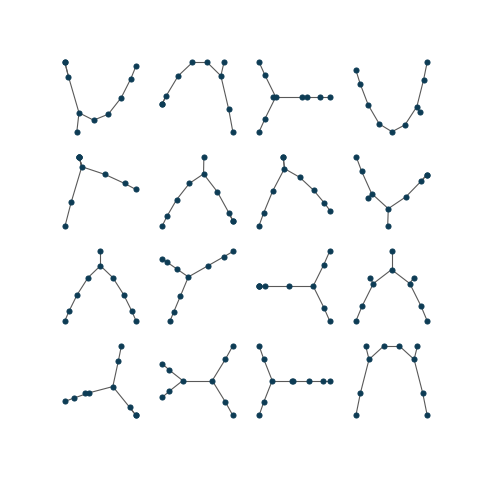
\includegraphics[scale=0.8]{Python/Figures/Tree-sample10.png}
	\caption{Maximal tree chosen randomly with uniform distribution among all the possible ones in complete graph (10) of vertices.}
	\label{fig:RandromTrees}
\end{figure}

The expected execution time of the algorithm per tree is equal to $\E(C_{s})$. It is known that for the connected graph $\E(C_{v}) = O(n^{3})$, nevertheless in \cite[Broder, Andrei 89]{boundsoncovertime} there is a proof that if the transition matrix of a random walk have the second greater eigenvalue bounded away from 1, then the expected covering time is only $O(n\cdot log(n))$. Almost every graph in the Erdös-Rényi model satisfy this condition when $p > \frac{c\cdot log(n)}{n}$, in particular when $p=\frac{1}{2}$ and for almost every d-regular graphs \cite[Friedman 89]{secondEigenValue}. 
In the figure \ref{fig:tiemposGEN} appear the results of the execution time of the implemented algorithm.
\begin{figure}[h!]
	\centering
	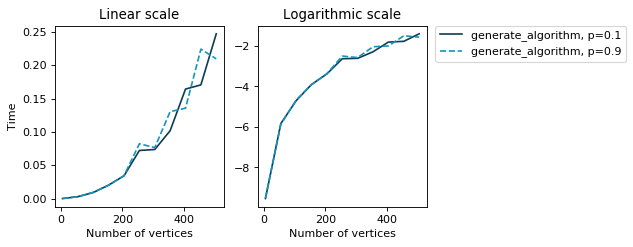
\includegraphics[scale=0.8]{Python/Figures/Time-execution-generate-algorithm.png}
	\caption{ Execution time of the algorithm in seconds varying the size of the tree. It appears the normal and the logarithmic scale}
	\label{fig:tiemposGEN}
\end{figure}
